%!TEX root = ../thesis.tex
In this chapter we will attempt to bring together some of the ideas that has laid the ground and motivation for our thesis work.
Our process has not been on an entirely straight line, so at the same time we will try to draw lines between the different areas and disciplines that have shaped and influenced our process and ideas into the end result we present in this thesis.  

The original basis for this thesis was born from a fascination of things that \emph{moves, adapts and changes} - the bringing of ``life'' to the objects and environments that surrounds us, letting them transform to our needs, both in function and form. 

The fascination of giving life to inanimate objects is not entirely new.
A famous example of this is the Vaucanson Duck, an automata created by the French inventor and artist Jacques Vaucanson in 1739 \citep{riskin2003defecating}.
It was later depicted by a nineteenth-century inventor, as seen in figure~\ref{vaucanson_duck} 
The mechanical duck, which supposedly contained over a thousand parts, could both flap its wings and appeared to have the ability to eat, digest, and defecate grains.

The animation of `things' still amazes today, both in the world of technology, with advancements in robotics, and in the world of crafts where ingenuity and craftsmanship can give rise to fascination.   
An example of the latter is Theo Jansen's that gives life to new species of animals with his amazing Strandbeests \cite{strandbeestJansen}.  
Made mostly from yellow plastic tube and fabric sails, these skeletons traverses the beaches of the Netherlands, living off the wind, adapting to the turnings of the elements, see figure~\ref{strandbeest}.

\begin{figure}[h]
	\centering
	\begin{minipage}{.45\textwidth}
		\centering
		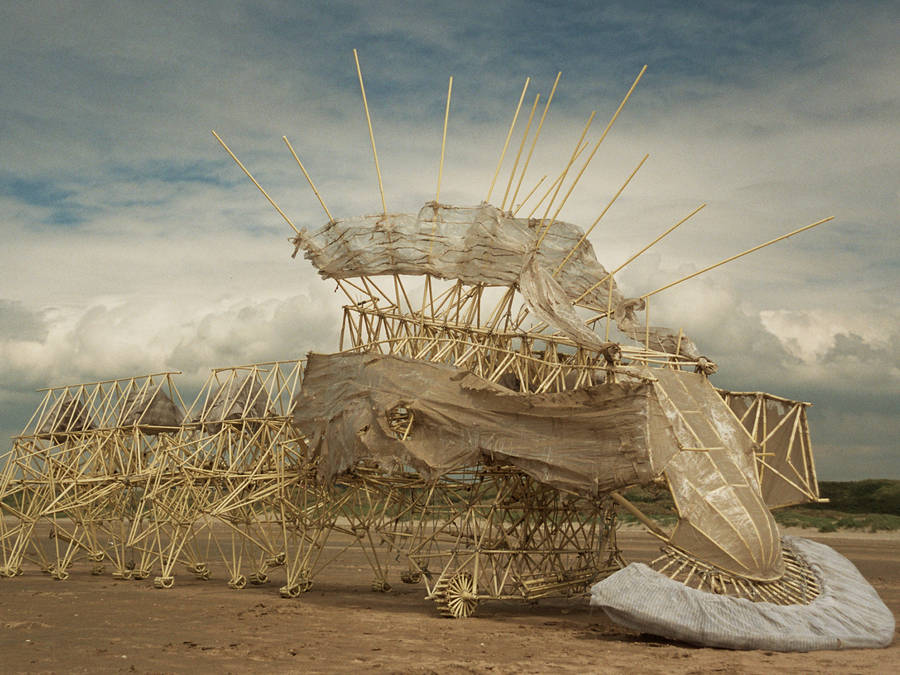
\includegraphics[width=0.9\linewidth]{figures/strandbeest}
		 \captionof{figure}{One of Jansen's Strandbeests, \citep{strandbeestJansen}}
		\label{strandbeest}
	\end{minipage}%
	\hspace{0.1cm}
	\begin{minipage}{.45\textwidth}
		\centering
		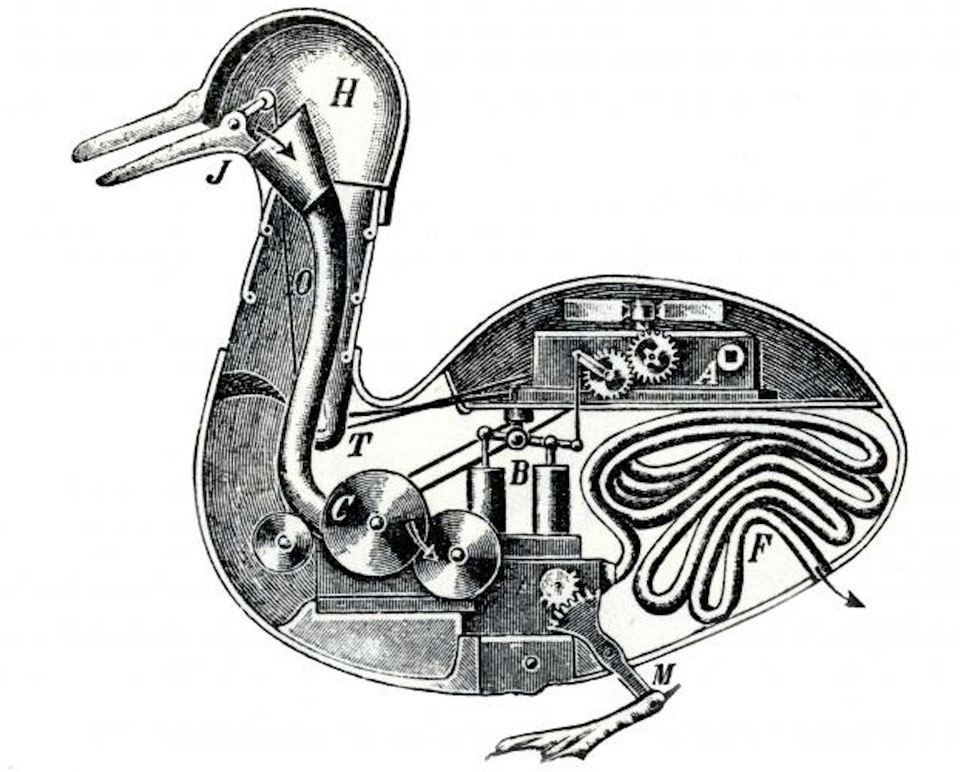
\includegraphics[width=0.9\linewidth]{figures/vaucanson_duck}
		\captionof{figure}{A nineteenth-century inventor's imagined depiction of the inner workings of the Vaucanson Duck \citep{riskin2003defecating}}
		\label{vaucanson_duck}
	\end{minipage}	
\end{figure}

These two examples, each impressive in their own right, points to the powerful expressiveness that actuation can give objects, as we have a tendency to relate things that move to living entities. 
\blank  
Looking back at traditional computing systems, before the era of Ubiquitous Computing \citep{weiser1991computer}, there has been a strong separation between the digital bits and the material world surrounding us.
The tangibility of digital information was then, for the most part, limited to keyboards and mice, icons and windows. 
And even though metaphors and graphical representations has helped us visualize the digital matter that flow through the transistors, these digital bits, when presented to the physical world, still only manifests as pixels on a screen, intangible and transient. 
\citet{ishii1997tangible} vision of Tangible Bits, along with Weiser's ubiquitous computing, was a break away from the traditions, where the goal was to create a strong coupling from the digital bits of the computer to the physical environments we surround ourself with.

One of the powerful abilities of digital interfaces is still lacking, or is at least not articulated much, in the concept of tangibles. 
Digital information and digital interfaces have, due to their intangible and transient nature, a degree of malleability and adaptability that are not found in the physical objects that we surrounds us with, making a complete transition between the digital and the physical hard to achieve. 
\blank
In 1965, Ivan Sutherland presented a vision of what he called the Ultimate Display \citep{sutherland1965ultimate}, envisioning a room where digital bits would control the existence of matter, completely removing the boundaries between the two worlds.
This display would attain the palpability of the physical world as well as the transience of the digital, as it would let digital information manifest itself into physical objects.
This is, of course, still only a vision, but in recent years there has been an increasing interest in bridging the gaps that still exists between the two worlds, such as physical malleability and transience.
Under different names such as kinetic interaction, organic user interfaces, actuated interfaces, shape-changing interfaces and programmable matter, researchers has attempted to get closer to creating truly ubiquitous systems.    
This has resulted in an increasing amount of of what \citet{coelho2009programming} calls `transient materials', such as flexible displays, shape-changing materials, e-textiles and sensor networks.
\blank
Interestingly some of these transient materials, especially e-textiles, have given rise to DIY communities that combines traditional crafts with electronics, inviting to a new form of material end-user-programming.
For example \citet{buechley2008lilypad}'s LilyPad Arduino which serves as a tool-kit for creating e-textile projects, Makey Makey\footnote{http://www.makeymakey.com/}, a tool-kit for tangible interaction, along with web communities such as Instructables\footnote{http://www.instructables.com/} and Make:\footnote{http://makezine.com/}.
DIY is interesting as a concept as it challenges the traditional balance between products and users making it possible for the consumer to create  or modify what he/she wants, instead of relying on the producer or designer to define what is wanted.
The DIY approach does somewhat democratize the product development as users are able to redefine or refit products to their needs, an approach that is also seen in the digital world with open-source software.
\blank
The idea of giving the control back to the user does also relate to the relationship between computers and user.
One of the areas of ubiquitous computing that have received a lot of focus is context-awareness.
First coined by \citet{schilit1994context}, context-aware computing focuses on letting the computer act based on contextual information.
But there is a tendency to exclude the user from the control-loop, as interaction possibilities, user intentions and actions are inferred from the sensed context, a context which might not correlate with what the user finds as the \emph{correct} one.
Implicit interaction is not necessarily a bad thing as it is the basis for many useful applications, especially in mobile computing, but we do believe that there is value in keeping the user in some degree of control
\blank
A domain where we find the relationship between computers and user interesting is the domestic environment.
An essential aspect of a home is the ability to make it one, in the sense that you, as an inhabitant, is able to modify it continuously to respond to your needs and desires as to what you want from your home.
As computers become an increasingly more integrated part of our everyday life, computers also have to be taken into account when we talk about the home.
Since the entrance of the personal computer into the home in the 80s much has happened.
Today we see deeply integrated `smart homes' where, in the extreme cases, even small changes to the house needs a call to a computer technician \todo{ref til dubai eller andet ekstremt eksempel?}.
The question is how to make computing systems in the home that are made to evolve and adapt and that functions on the premises of the inhabitants.  

\todo{mere her}
\blank
In the midst of all these seemingly divergent digressions we believe that there is an unexplored space for interfaces that focuses on adaptability and situational awareness, that function on the terms of the user and not the computer system, bringing a more dynamic relationship, as seen in software, into the world of physical interactable artefacts.

In this thesis we want to explore and expand on the concept of Ad Hoc Interfaces, a concept that has evolved and taken inspiration from all of the above mentioned areas, and more. 
\todo{some more} 

Noter:
\begin{verbatim}
Afslutte med en aabning til projektet - 
hvordan vi med udgangspunkt i ovenstaaende har bevaeget os videre,
hvad vil vi udforske.
\end{verbatim}